\documentclass[border=4pt]{standalone}
% Shared style for every diagram. Colour-blind-safe palette (Okabe-Ito).
\usepackage[T1]{fontenc}
\usepackage{helvet}
\renewcommand{\familydefault}{\sfdefault}
\usepackage{tikz}
\usetikzlibrary{arrows.meta,positioning,fit,backgrounds,calc,shapes.geometric,decorations.pathreplacing}
\definecolor{cblue}{HTML}{0072B2}
\definecolor{corange}{HTML}{E69F00}
\definecolor{cgreen}{HTML}{009E73}
\definecolor{cred}{HTML}{D55E00}
\definecolor{cpurple}{HTML}{CC79A7}
\definecolor{cgrey}{HTML}{6B7280}
\definecolor{csky}{HTML}{56B4E9}
\tikzset{
  >={Stealth[length=2.2mm]},
  box/.style={draw, rounded corners=3pt, align=center, minimum height=11mm, minimum width=22mm, font=\small, line width=0.7pt},
  real/.style={box, draw=cblue, fill=cblue!8},
  sim/.style={box, draw=corange, fill=corange!12},
  future/.style={box, draw=cgrey, dashed, fill=white},
  flow/.style={->, line width=0.8pt, draw=black!75},
  dflow/.style={->, line width=0.8pt, dashed, draw=cgrey},
  lbl/.style={font=\scriptsize, text=black!70},
  group/.style={draw=black!25, rounded corners=6pt, inner sep=6pt},
}

\begin{document}
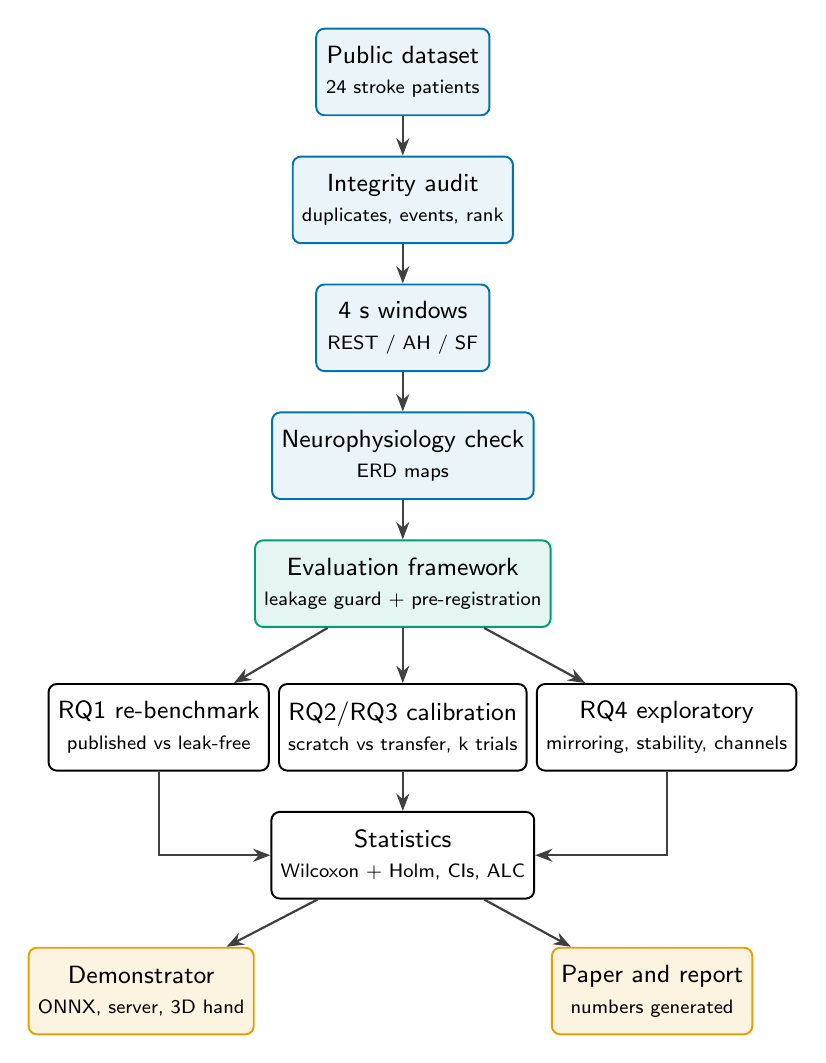
\begin{tikzpicture}[node distance=5mm and 6mm, every node/.append style={minimum width=30mm}]
  \node[real] (data) {Public dataset\\\scriptsize 24 stroke patients};
  \node[real, below=of data] (audit) {Integrity audit\\\scriptsize duplicates, events, rank};
  \node[real, below=of audit] (win) {4 s windows\\\scriptsize REST / AH / SF};
  \node[real, below=of win] (eda) {Neurophysiology check\\\scriptsize ERD maps};
  \node[box, draw=cgreen, fill=cgreen!10, below=of eda] (prereg) {Evaluation framework\\\scriptsize leakage guard + pre-registration};
  \node[box, below left=7mm and -2mm of prereg] (rq1) {RQ1 re-benchmark\\\scriptsize published vs leak-free};
  \node[box, below=7mm of prereg] (rq2) {RQ2/RQ3 calibration\\\scriptsize scratch vs transfer, k trials};
  \node[box, below right=7mm and -2mm of prereg] (rq4) {RQ4 exploratory\\\scriptsize mirroring, stability, channels};
  \node[box, below=of rq2] (stats) {Statistics\\\scriptsize Wilcoxon + Holm, CIs, ALC};
  \node[sim, below left=6mm and 2mm of stats] (demo) {Demonstrator\\\scriptsize ONNX, server, 3D hand};
  \node[sim, below right=6mm and 2mm of stats] (paper) {Paper and report\\\scriptsize numbers generated};
  \foreach \a/\b in {data/audit, audit/win, win/eda, eda/prereg} \draw[flow] (\a) -- (\b);
  \draw[flow] (prereg) -- (rq1); \draw[flow] (prereg) -- (rq2); \draw[flow] (prereg) -- (rq4);
  \draw[flow] (rq1) |- (stats); \draw[flow] (rq2) -- (stats); \draw[flow] (rq4) |- (stats);
  \draw[flow] (stats) -- (demo); \draw[flow] (stats) -- (paper);
\end{tikzpicture}
\end{document}
